% Chapter Template

\chapter{Implementation} % Main chapter title
%Possible solutions (in the context)
\label{Chapter4} % For referencing the chapter elsewhere, use \ref{Chapter1} 

After introducing the project as it existed before this thesis,
this chapter will concern the planning and implementation of the extension that was build.
The implementation used the aforementioned tools as well as some smaller libaries that will be explained in the following section.

\section{Project Design}
The project's design followed a design thinking approach.
The following shows the different steps that were taken that lead to the changes that were planned.

\begin{description}
	\item [Empathise]\hfill \\
	      As a first step, interviews and tests with the existing project were executed.
	      Orignially, the author wanted to build another riddle for the room.
	      It was quickly discovered that constraints would complicate that task.
	      Three people who had worked with the room reported they experienced severe difficulties
	      on trying to change the existing pattern.
	      Frequently mentioned was the overall lack of understanding the room as a whole.
	      Some parts, like the TCP-socket in Unity, were relatively easy to modify, others, like the riddles themselves were disclaimed
	      "not to be touched or they might break".
	      As the room had many visitors (a few a hours a day, 2-4 times a week), changes which would affect the look
	      of the room or make it unstable for a longer period of time were not welcomed.

	      In the time following these interviews,
	      a deeper occupation with the project seemed necessary to develop alternative ideas for this thesis.
	      The author's impression was that the project lacked documentation and explanations on many sides.
	      Understanding the processes and the different parts of communication proved to be difficult,
	      as it didn't seem to follow any standartized structure or protocol.
	      The result of this examination is further explained in Chapter \ref{Chapter3}.

	      On questioning the former architect about his choices,
	      he stated that the project was build under time pressure
	      and everything was therefore implemented best to the architect's knowledge,
	      but without further scientific research or extensive planning.

	\item [Define]\hfill \\
	      The "Empathise" stage lead to the impression that a new riddle
	      would be considered "nice-to-have" whereas
		  extensions to improve the flexibility and comprehensibility of the room would be welcomed.
		  Derived from the workload anyalysis in Chapter \ref{Chapter3},	 
	it was determined that the cognitive and memory work required from a developer were the most critical points
	that one might spend a lot of time on, or might decide not to join the project at all.
	It was defined that:

	To reduce cognitive (C) work, the process of learning and discovering the project must be simplified.

	To reduce the memory (M) work, the amount of commands to remember to control the room must be reduced and the start-up of the room must be simplified.

	\item [Ideate]\hfill \\
	The next step was to devise ideas and to estimate their workload to decide 
	which should be included in the prototype. Since the author had little experience as a software developer,
	complicated coding tasks (judged by the author's supervisor) were cut, 
	like a graph-editor for the front-end.

	After discussing possible approaches, a few specific tasks were set:
	      \begin{enumerate}
		      \item Developing a web interface that would:
		            \begin{itemize}
			            \item Enable more overview and control for the existing riddles (M)
			            \item Ease the testing process for new riddles by displaying them dynamically (C)
			            \item Allow remote access (P) and control (C) within the lokal w-lan enviroment
		            \end{itemize}
		      \item Retrieving information from the room must work automatically, therefore should the "feedback mode" be enabled on start-up (M)
		      \item Providing a thorough documentation for future developers  (C/M)
	      \end{enumerate}

	      The summarized goals for improvement in the different areas can be seen in \ref{fig:workload}.

	      \begin{figure}[th]
		      \centering
		      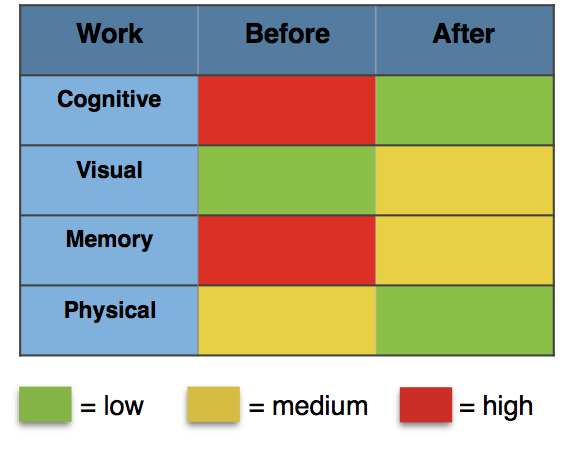
\includegraphics[width=50mm,scale=.5]{Figures/workload}
		      \decoRule
		      \caption[workload]{Workload of the different aspects color-coded}
		      \label{fig:workload}
	      \end{figure}

	\item [Prototype]\hfill \\
		 Afterwards, prototyping began. 
		 The development process of the prototype is explained in the following sections of this chapter.
	    Proof of Concepts were designed for each stage of the implementation (\ref{fig:PoC}).
	\item [Test]\hfill \\
		  Testing happened regulary at least once a month, later every two weeks.
		Extensive testing was difficult to achieve, as the room did not provide 
		   an internet connection needed to install modules (e.g. Node.js) on the PC 
		   and missed basic testing tools like a coding enviroment. 
		   Additionaly, due to the room's physical set-up, testing directly on the PC turned out 
		   to be inconvenient. The PC was hidden behind a wall and difficult to access, 
		   which meant mouse and keyboard could barely reside outside the wall's recess.
		   Consequently, most testing was conducted on two laptops brought by the author: 
		   One Macbook Pro from 2009 with OSX 10.11.6, and a Windows laptop with Windows 10 installed.
		   Throughout testing, new features were designed and iterated.
\end{description}

Our final result is a MVP %Reference abkürzung 
which provides the bare functionalites but lacks in design 
and more extensive features which we will eleborate in the evaluation.

\begin{figure}[th]
	\centering
	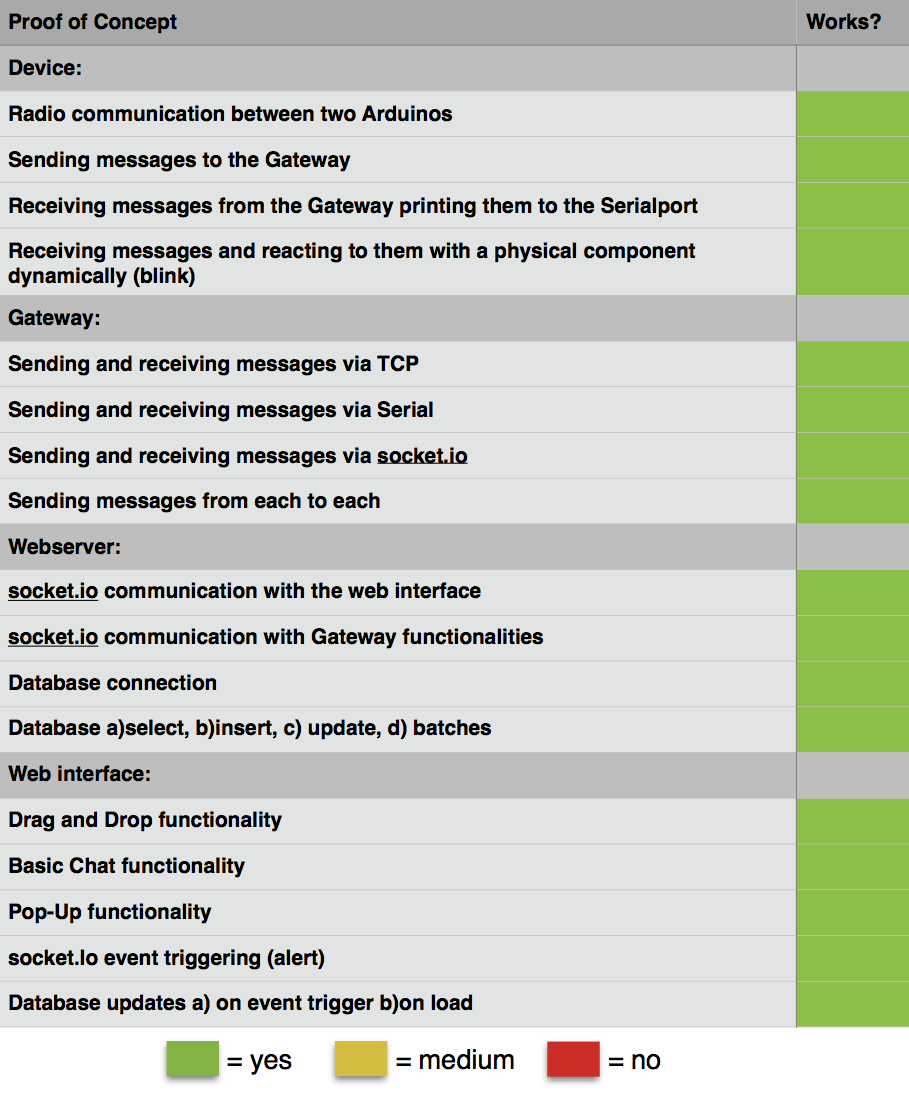
\includegraphics[width=100mm,scale=1]{Figures/PoC}
	\decoRule
	\caption[PoC]{List of our PoC steps}
	\label{fig:PoC}
\end{figure}


\section{Architecture}

As mentioned earlier, IoT-Projects typically follow a SoA %Reference to abkürzung!
to keep the project flexible and expandable.

The goals were set with that architecture in mind and resulting architecture changes
designed to become loosely coupled to encourage improving a specific module of the project.

The changes were meant to reflect concepts of a SoA, creating self-contained,  
reusable and loosely coupled components
to encourage improving a specific module of the project on demand.

For example, the TCP- and serial-connection were set-up in a general way (send/ receive all) 
to separate the data processing from the transport channels. 

Also, communication was designed not interfere with other each other, e.g. 
communication to Unity should still work if a connection to the front-end failed.

For that reason, a backend was implemented which ensured reliable data storage.

In that way, changes reflect the composition of a fog architecture, 
though there is no cloud available or planned which is an important part 
of larger IoT project architecture.

The front-end connection received it's own namespace for Socket.io events so front-end relevant data
would only be proccessed in it's set namespace component.

\begin{sidewaysfigure}
	\centering
	\includegraphics[width=200mm,scale=2]{Figures/escapeUmlNew}
	\caption{The new escape room architecture}
	\label{fig:newEscapeUml}
\end{sidewaysfigure}
%picture of our architecture

\section{Device}
Since the room consisted of microcontroller-driven-riddles only at the time of this thesis, 
we decided to design a prototype and a template for integration of future microcontroller-driven-riddles.
The principle concepts though are appliable to any device.

\subsection{RFM69HCW Wiring}
As most riddles are connected to RFM69HCW modules manually, the first set-up of the prototype 
consisted of an Arduino Uno connected to a RFM69HCW. As one can see in Figure \ref{fig:prototypeV1},
the wiring looks chaotic.



Later, the set-up was replaced with an Adafruit Feather 32u4 which is a microprocessor with an integrated 
RFM69HCW module an therefore reduces the complexity of the wiring needed for the riddle.
This prototype included an external battery as the Feather doesn't support 5V output.
The Adafruit Feather 32u4 needs an external libary to work, the only difference though (apart from the radio set-up)
is the assignment of the SPI lines.

\begin{figure}[H]
	\centering
	\includegraphics[width=75mm,scale=.75]{Figures/prototypeV1}
	\decoRule
	\caption[prototypeV1]{Prototype, Version 1}
	\label{fig:prototypeV1}
\end{figure}


\begin{figure}[H]
	\centering
	\includegraphics[width=50mm,scale=.5]{Figures/prototypeV2}
	\decoRule
	\caption[prototypeV2]{Prototype, Version 2}
	\label{fig:prototypeV2}
\end{figure}

\subsection{Template}

The template was designed to simplify the process of developing a riddle.
The escape room provided in its prior form no support for new riddle-developers.
We decided to modify the existing communication protocol, 
but had to be careful not to impact communication to the existing riddles.

Still, we wanted simplify the communication system for riddle-developers.

The existing communcation protocol followed a "string-to-chararray-send" and "receive -chararray-to-string" structure that we applied to our implementation.
In contrast to the existing puzzles though, we decided to separate the code into several parts, named by the functionality they supplied.

%Chararrays are smaller than strings hence faster for radio-communication.
The template is devided into 3 parts: "Groundwork", "Riddlefunctionality" and "Remote Functionality".

\begin{description}
	\item [Groundwork]\hfill \\
	      Section to be filled with libaries, variables and definitions.
	\item [Riddle Functionality]\hfill \\
	      To contain the riddles functionalities separated from nearly any communication.
	      The only communication that needs to be defined there is when the Microcontroller should send messages and which.
	      That is executed by writing a single line command containing the desired string.
	      If the string's value is defined in the "registerRiddle()" function of the "Remote Functionality" section, it will be translated in the web interface.

	\item [Remote Functionality]\hfill \\
	      To contain any remote commands for interaction with the web interface and the server.
	      The "Remote Functionality" section consists of two functions:
	      \begin{description}
		      \item [registerRiddlle()]\hfill \\
		            Here is where strings to be send once on starting the device are defined.
		            These strings set the configuration of the variables in the web interface.
		            To work, they need to follow a specific structure:
		            \begin{enumerate}
			            \item an Index for the riddlevariable (to order the variables)
			            \item a "readonly" or "write" command (to make it static or dynamic)
			            \item the name of the variable (to translate)
			            \item the value of the variable (needs to be converted into a String)
			            \item an optional button value (if it was present, a button would show)
		            \end{enumerate}
		            That structure is meant to be applieable for any variable.
		      \item[remoteCommand()]\hfill \\
		            Designed to contain processing of incoming messages from the gateway/PC.
		            It's connected to the radio functionality further down in the code, nevertheless allows the user not to care about how the messages are processed.

		            The developer is advised to use a "Switch-Case" structure to define the microcontroller's reactions to radio messages, to keep the processing clean and standartized.
		            For any reaction concerning the defined variables, the case should match the index of the variable in order for the buttons within the web interface to work.

	      \end{description}

\end{description}



\begin{figure}[th]
	\centering
	\includegraphics[width=75mm,scale=0.75]{Figures/registerRiddle}
	\decoRule
	\caption[registerRiddle]{"registerRiddle" definition in the Arduino IDE}
	\label{fig:registerRiddle}
\end{figure}

%fig arduino def

The documentation provided explains the template in further detail.

\subsection{Prototype}

For our prototype, an Arduino Uno with a RFM69HCW module, a keypad, and an I2C-display were used.
All the parts required specific libaries.
%Pictures of syntax and libaries
The riddles challenge would be to guess a code and enter it.
The use case would be that a riddle could to provide different difficulties by adjusting the codes length.
Moreover would the riddle possess static  "won", "lost", and "reset"-values to track and control the riddle's state.
%prototype pic

\section{Back-End}
PostgresSQL was used and the relational model implemented for the back-end.
Two tables were enough to fit our needs.
One table manages the location, name and other general information about the riddle displayed in the main view,
whereas the other one is responsible for saving and editing the information displayed in the pop-up window.
The key predicate was the id of the riddle, which was common to both tables.
This seperation simplifies database changes, clearifying the tasks happening on the Node.js server.
The Node.js server connects the information when sending to the front-end by assigning the details with the riddle's id to the corresponding riddle.

%Database schema einfügen
\section{Middleware}

\subsection{Web Server}
It quickly became apperant that the middleware web server would use Node.js due to the reasons mentioned in \ref{Chapter2}.
The decisive factor for this decision was that it would be easier to develop and understand a web server programmed in the same language as the front-end.

As all the website operations were processed on the client-side, Node.js main operation was the database and handling.
The "pg-promise" libary \parencite{pg-promise} was used for database integration with PostgreSQL.

Depending on the event emitted by the web interface, database-queries to select, update or delete entries could be triggered.

If the gateway emitted a message, a control mechanism would check if the riddle was known and either add a new riddle, update an existing riddle (if new variables where recognized) or translate the incoming data .

With Socket.io, the client would register whether a front-end or another client would register and forward the needed data from the database.
By namespacing (creating different channels for different clients), we tried to avoid dispensable traffic.
The gateway would receive the changeable ("write") values and send them to the connected riddles.
The front-end would receive the sorted database data in a sorted json fit to the front-ends data-handling.

%Architecture We tried to implement our functionalities as loosely as possibilities, so 
\subsection{TCP/Serial/Socket.IO-Client}
This part of the middleware changed several times during our development process.

Since the front-end allowed a reassignement of the messages that would trigger an Unityevent, 
filtering the incoming serial-messages before they were sent to Unity via TCP was required.

Furthermore would they need to be checked for eventual new riddleinformation or messages to be translated or displayed in the front-end.

Consequently, this part of the middleware would filter relevant "Finish"-serialmessages through a PostgreSQL-database, 
and activate a "checkSerialMessage" function which would decide on further processing.

First was tried to use the existing C++-server for the architecture but quickly discovered that understanding and extending the existing code would probably take longer than recreating the features.

Then, because many developers within the faculty were proficient in C\# from Unity development, an implementation the functionalites was tried with a .NET WPF-App.
This proved to be difficult, as it required multi-threading and communication between the threads. 
Both are well documented at the MSDN \parencite{MSDN},
however due to the mass of different techniques it was hard to get an overview.

The resulting code was easier than the C++ code, though not comparable to the readability of the Javascript-code of the Node.js implementation.
It took roughly a week to implement the desired functionalites.

Finally, the  C\# code was revisited and implemented it in Javascript to compare the workload and readability.
The same functionalites took about 10 hours to implement, though the author did by then have little experience in Javascript and started the C\# implementation with Unity-C\#-Knowledge.
The async-capabilities of Node.js revealed a tremendous advantage compared to the threading difficulties experienced with the .NET project in this project.


\begin{figure}[th]
	\centering
	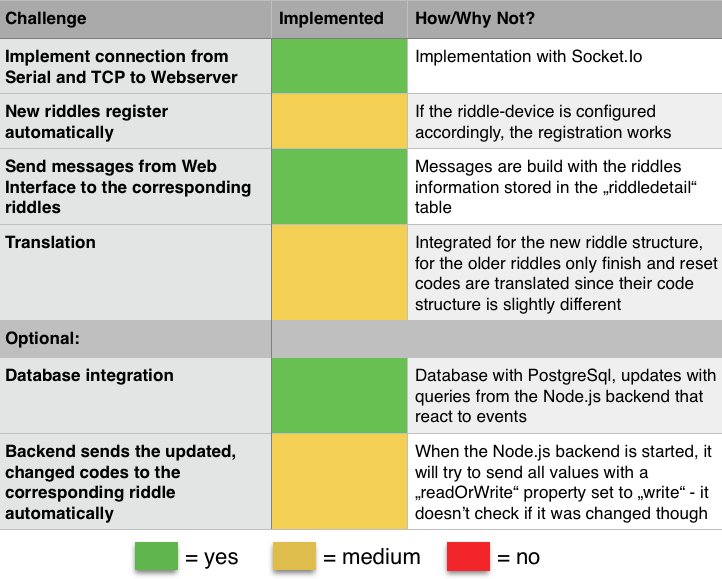
\includegraphics[width=100mm,scale=1]{Figures/backendOverview}
	\decoRule
	\caption[PoC]{Overview of the back-end challenges}
	\label{fig:BackEndTable}
\end{figure}


\section{Front-End}
For setting up our front-end, the Create-React-App was used, which provides a front-end build pipeline with Babel and Webpack.
React recommends to start there for single-page applications \parencite{createReactApp}.

It provides a package.json file in which modules and their versions are defined and set.
This prevents unwanted updates so the existing code won't risk becoming deprecated.

The npm packet manager (which is the standard packet manager for Node.js) automatically generates a package-lock.json file which saves the dependency tree in further detail.

For the file-structure, the recommended approach to group by filetype \parencite{reactStructure} in combination with the Create-React-App-structure was used.
%Fig: Our File structure front end

Starting out, it was planned to implement a node-editor to connect riddles in all thinkable ways.
Wheile listing the wished functionalities (Changeable riddleassignments with "Single", "AND" and "OR" connections to the Unity-Events) it was decided that a drag-and-drop table would supply those functionalites (Changeable assignements, OR connections) without creating a difficult User-Interface.
The React-dnd libary \parencite{reactDND} was used to implement the drag-and-drop functionality in React. 
Currently, it is not mobile-optimized since that was thought to be the less popular use case, but adding a mobile implementation for the module is possible.

When a user dropped a riddle into a "Video" field (and saved), the riddle's "Finish"-command would be reassigned on input to the corresponding Video-Trigger-command.
For example, the "Video1" command was originally triggered by "Riddle1".
If a user wanted to make "Riddle2" trigger "Video1", he needed to replace "Riddle1" in the "Video1"-List with "Riddle2".
Whenever "Riddle2" would now signal it's finished, the "Finish"-code of "Riddle1" would be sent to Unity via TCP.

If a Riddle was newly registered, it would be named "NewRiddle" and appear in the "Unassigned Riddles"-List on the web interface.
We designed an "Edit"-function which enabled changing the name of the riddle and deleting it in case it got corrupted (or deleted in real-life).

Another aspect was the popup-window for the riddles. It was planned to show enough information, yet keep it simple.
Consequently, our layout for the popup-window was designed flexibly to adapt to a desirable output depending on the usecase:

Each variable would be displayed in respect to its in the Arduino defined values.
If a variable was set "readonly", but didn't have a button value defined, the information would be listed plainly.
If a variable was set "write", but didn't have a button value defined, the information would be listed plainly.
Additionaly, an input field would enable changing the defined value and sending it to the Arduino automatically next time the Server would start.

If the microcontroller was programmed to interpret the incoming value, a variable could be changed that way (e.g. a password in a riddle).
If a button component was set in a variable, a button would appear instead of plain information about the variable.
The user would be able to click the button to send the code immediately to the riddle.
This functionality was especially designed with "Finish" and "Start" functionalities in mind, where a supervisor of the escape room might want to trigger these functionalites during a game if customers get stuck.

To increase the general overview for a supervisor, the color of a riddle would change to green once it's "Finish"-code arrived.

\begin{figure}[th]
	\centering
	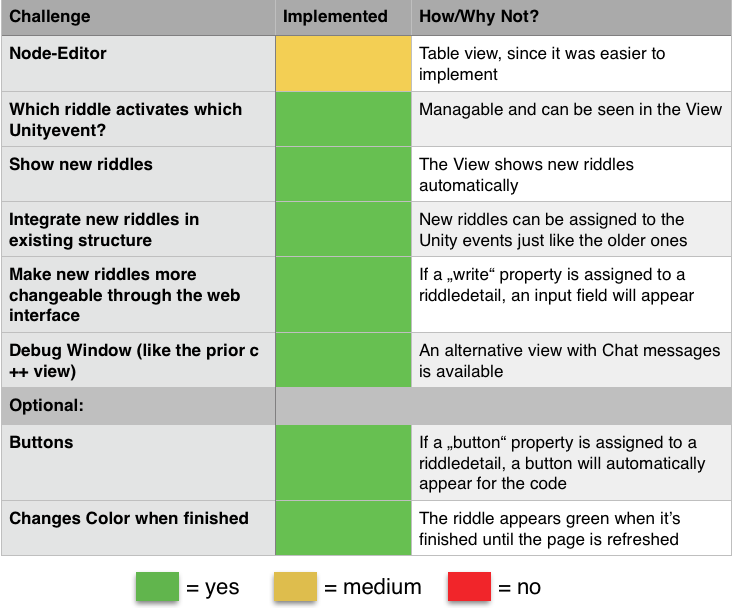
\includegraphics[width=100mm,scale=1]{Figures/frontendOverview}
	\decoRule
	\caption[FrontViewTable]{Overview about our front-view tasks.}
	\label{fig:FrontViewTable}
\end{figure}



